\documentclass[preview]{standalone}
\usepackage{xparse}
\usepackage[all]{genealogytree}
\usetikzlibrary{decorations}
\usetikzlibrary{positioning}
\usetikzlibrary{decorations.pathreplacing}
\tcbuselibrary{listings}

% This is enabled via xparse
% Setting the 2 colors is \internalnodes[pink][yellow]
\NewDocumentCommand{\internalnodes}{O{magenta} O{green} m}{%
\begin{tcbclipinterior}
	\fill[ #1 ] ([xshift=-3mm] interior.center) circle (2mm);
    \fill[ #2 ] ([xshift=3mm] interior.center) circle (2mm);
\end{tcbclipinterior}
}

\begin{document}

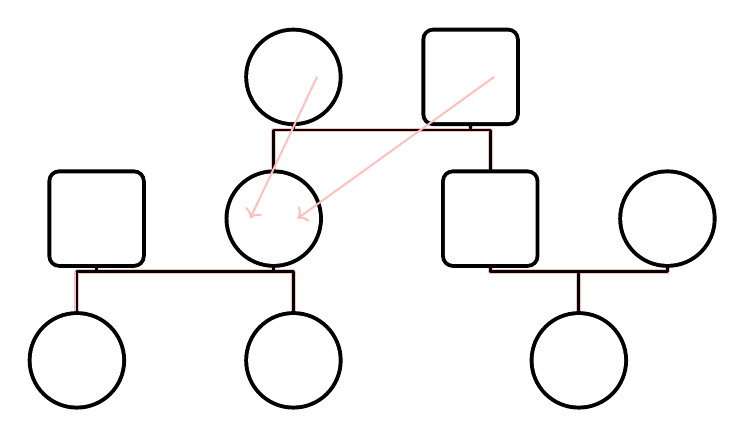
\begin{tikzpicture}
    \genealogytree[
        template=formal graph,
        tcbset={male/.style={colback=white,colframe=black,width=1.25cm,height=1.25cm},
        female/.style={circular arc,colback=white,colframe=black,width=1.25cm, height=1.25cm}},
        edges={anchoring=center,foreground=black,background=pink},
        level distance=1cm,
        parent distance in child graph=1cm,
        child distance in child graph=1.5cm
        ]{
        child[id=gparental]{
			g[id=gma,female,box={underlay={\internalnodes}}]{}
        p[id=gpa,male, box={underlay=\internalnodes}]{}
        child[id=parental] {
            p[id=dad,male]{}
            c[id=sib,female]{}
            c[id=you,female]{}
            g[id=mom,female,box={underlay=\internalnodes}]
            {}
        }
        child[id=cousins]{
        g[id=uncle,male]{}
        c[id=cousin,female]{}
        p[id=aunt,female]{}
        }
    }
    }
    \draw[->, pink, line width=0.25mm] ([xshift=3mm] gpa.center) --  ([xshift=3mm] mom.center);
    \draw[->, pink, line width=0.25mm] ([xshift=3mm] gma.center) --  ([xshift=-3mm] mom.center);
    % \node[] at (gpa) {Poop};
\end{tikzpicture}

\end{document}



